\begin{figure}[h!]
   \centering
   \begin{subfigure}[b]{0.4\textwidth}
      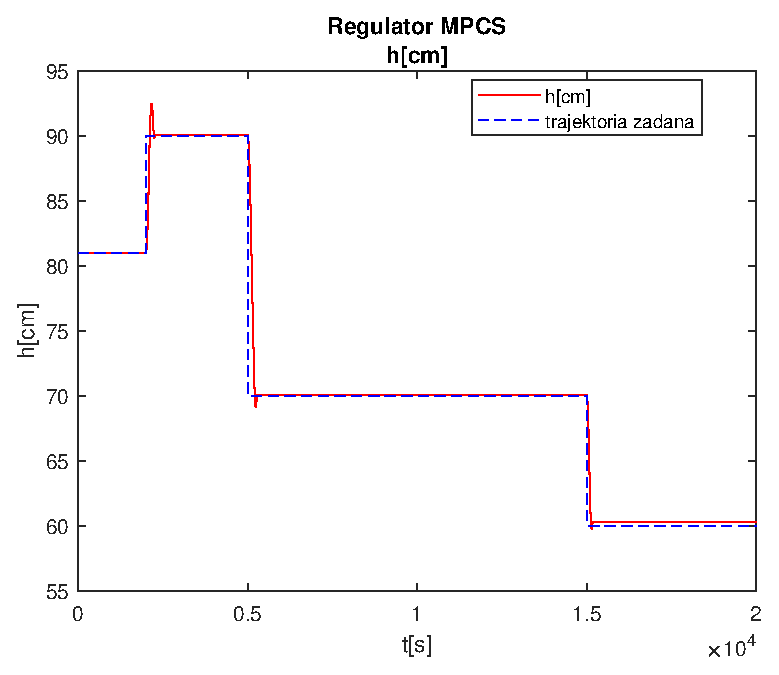
\includegraphics[width=1\linewidth]{img/MPCSanaRK/MPCSRKHN50Nu10l100.eps}
      \caption{}
      \label{fig:fig:MPCSRKN50Nu10l1001}
   \end{subfigure}
       
   \begin{subfigure}[b]{0.4\textwidth}
      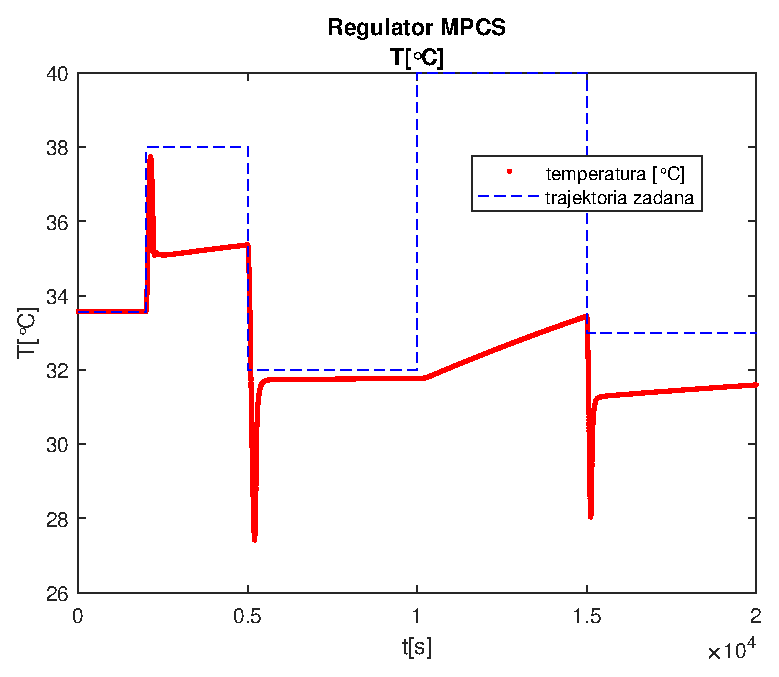
\includegraphics[width=1\linewidth]{img/MPCSanaRK/MPCSRKTN50Nu10l100.eps}
      \caption{}
      \label{fig:fig:MPCSRKN50Nu10l1002}
   \end{subfigure}
       
   \begin{subfigure}[b]{0.4\textwidth}
      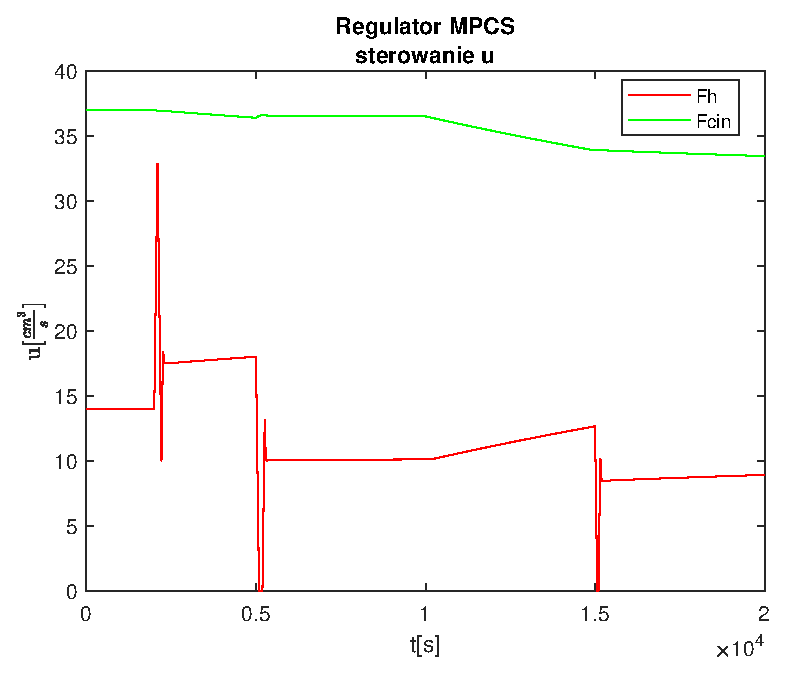
\includegraphics[width=1\linewidth]{img/MPCSanaRK/MPCSRKControlN50Nu10l100.eps}
      \caption{}
      \label{fig:fig:MPCSRKN50Nu10l1003}
   \end{subfigure}
       
   \caption{Wykresy dla regulatora MPCS, obiekt nieliniowy.}
   \label{fig:MPCSRKN50Nu10l100}
\end{figure}
           
